\PassOptionsToPackage{unicode=true}{hyperref} % options for packages loaded elsewhere
\PassOptionsToPackage{hyphens}{url}
%
\documentclass[]{article}
\usepackage{lmodern}
\usepackage{amssymb,amsmath}
\usepackage{ifxetex,ifluatex}
\usepackage{fixltx2e} % provides \textsubscript
\ifnum 0\ifxetex 1\fi\ifluatex 1\fi=0 % if pdftex
  \usepackage[T1]{fontenc}
  \usepackage[utf8]{inputenc}
  \usepackage{textcomp} % provides euro and other symbols
\else % if luatex or xelatex
  \usepackage{unicode-math}
  \defaultfontfeatures{Ligatures=TeX,Scale=MatchLowercase}
\fi
% use upquote if available, for straight quotes in verbatim environments
\IfFileExists{upquote.sty}{\usepackage{upquote}}{}
% use microtype if available
\IfFileExists{microtype.sty}{%
\usepackage[]{microtype}
\UseMicrotypeSet[protrusion]{basicmath} % disable protrusion for tt fonts
}{}
\IfFileExists{parskip.sty}{%
\usepackage{parskip}
}{% else
\setlength{\parindent}{0pt}
\setlength{\parskip}{6pt plus 2pt minus 1pt}
}
\usepackage{hyperref}
\hypersetup{
            pdfborder={0 0 0},
            breaklinks=true}
\urlstyle{same}  % don't use monospace font for urls
\usepackage[margin=1in]{geometry}
\usepackage{longtable,booktabs}
% Fix footnotes in tables (requires footnote package)
\IfFileExists{footnote.sty}{\usepackage{footnote}\makesavenoteenv{longtable}}{}
\usepackage{graphicx,grffile}
\makeatletter
\def\maxwidth{\ifdim\Gin@nat@width>\linewidth\linewidth\else\Gin@nat@width\fi}
\def\maxheight{\ifdim\Gin@nat@height>\textheight\textheight\else\Gin@nat@height\fi}
\makeatother
% Scale images if necessary, so that they will not overflow the page
% margins by default, and it is still possible to overwrite the defaults
% using explicit options in \includegraphics[width, height, ...]{}
\setkeys{Gin}{width=\maxwidth,height=\maxheight,keepaspectratio}
\setlength{\emergencystretch}{3em}  % prevent overfull lines
\providecommand{\tightlist}{%
  \setlength{\itemsep}{0pt}\setlength{\parskip}{0pt}}
\setcounter{secnumdepth}{0}
% Redefines (sub)paragraphs to behave more like sections
\ifx\paragraph\undefined\else
\let\oldparagraph\paragraph
\renewcommand{\paragraph}[1]{\oldparagraph{#1}\mbox{}}
\fi
\ifx\subparagraph\undefined\else
\let\oldsubparagraph\subparagraph
\renewcommand{\subparagraph}[1]{\oldsubparagraph{#1}\mbox{}}
\fi

% set default figure placement to htbp
\makeatletter
\def\fps@figure{htbp}
\makeatother


\title{\textbf{Automatisation de l'étude de la croissance des coraux par
photogrammétrie}}
\author{par Orlane VELIN}
\date{11/16/2021}

\begin{document}
\maketitle

\hypertarget{table-des-matiuxe8res}{%
\subsubsection{Table des matières}\label{table-des-matiuxe8res}}

\begin{enumerate}
\def\labelenumi{\arabic{enumi}.}
\item
  \protect\hyperlink{introduction}{Introduction}

  \protect\hyperlink{partieI}{I- Changement global et impacte sur récifs
  coralliens}

  \protect\hyperlink{partieII}{II- Enjeux socio-écologique lié aux
  écosystèmes coralliens global}

  \protect\hyperlink{partieIII}{III- Les techniques de mesure de la
  croissance corallienne}

  \protect\hyperlink{partieIV}{IV- Cadre de l'étude}
\item
  \protect\hyperlink{Matuxe9rielux5cux2520etux5cux2520muxe9thodes}{Matériel
  et méthodes}
\end{enumerate}

\hypertarget{introduction}{%
\subsubsection{Introduction }\label{introduction}}

\hypertarget{i--changement-global-et-impacte-sur-ruxe9cifs-coralliens}{%
\paragraph{I- Changement global et impacte sur récifs coralliens
}\label{i--changement-global-et-impacte-sur-ruxe9cifs-coralliens}}

Depuis les années 50, un changement global du climat s'effectue à
l'échelle de la planète. L'augmentation de l'activité anthropique est en
effet responsable d'une importante émission de gaz à effet de serre dans
l'atmosphère. On estime que 33\% de ces gazs seraient absorbés par les
océans chaque année (Woolf et al. 2019). Responsable d'une acidification
des océans, l'augmentation du CO2 dissout et de l'acide carbonique
aurait provoqué une baisse de 0,1 du pH des eaux de surface depuis l'ère
industrielle. Les tendances à cette diminution varieraient entre 0,0014
et 0,0024 par an (Diouf 2016). Dans une étude menée sur les eaux
Nord-Ouest de la Méditerranée en 2017, des chercheurs ont montré, que la
modification du pH est liée à 60\% à la quantité de CO2 absorbée et à
40\% à la température de l'eau (Kapsenberg et al. 2017). Or, avec le
réchauffement atmosphérique, un renforcement de l'effet de serre naturel
conduit à une hausse de la température moyenne de l'eau. Dans un rapport
de 2021, le GIEC (Groupe intergouvernemental d'experts sur l'évolution
du climat) prévoit une augmentation de la température moyenne de l'air
de 1,5 °C d'ici 2030 (Coste et al. 2021), entraînant un réchauffement
encore plus important de la surface des océans.

Au niveau des récifs coralliens, ces phénomènes sont principalement
responsables d'un blanchissement massif des récifs à l'échelle mondiale.
Le stress écologique provoque une rupture de la symbiose entre les
polypes de coraux et les zooxanthelles, privant ainsi la colonie de
l'apport en nutriment que lui fournit la microalgue avec la
photosynthèse. Si la température reste élevée, la symbiose n'est pas
renouvelée et la colonie meurt, laissant son squelette calcaire
apparent. Bien que les coraux soient capables de récupérer d'un épisode
de blanchissement qui ne persiste ou ne s'intensifie pas, il a été
montré que le stress mène à la mort dans 50\% des cas, entrainant alors
une baisse importante de l'abondance des récifs (Dokken 2014). D'après
les prévisions du GIEC, on peut s'attendre à une multiplication des
épisodes de blanchissement et une modification conséquente de
l'écosystème corallien dans les années à venir. La baisse du pH a
également des conséquences sur les fonctions physiologiques des coraux.
Elle diminue la disponibilité des ions Calcium de l'eau de mer
entrainant sa saturation de l'aragonite. Pour les coraux durs cela
implique une cristallisation plus difficile du minéral pour construire
leur squelette calcaire (Shaw et al. 2015). Les coraux ne présentent pas
tous la même sensibilité à la modification de leur milieu et leurs
réponses aux perturbations varient entre les espèces. De ce fait, une
conséquence de l'acidification pourrait être de réduire la complexité
des récifs en diminuant la diversité des espèces composant les récifs
coralliens (Darling et al. 2012).

\hypertarget{ii--enjeux-socio-uxe9cologique-liuxe9-aux-uxe9cosystuxe8mes-coralliens-global}{%
\paragraph{II- Enjeux socio-écologique lié aux écosystèmes coralliens
global
}\label{ii--enjeux-socio-uxe9cologique-liuxe9-aux-uxe9cosystuxe8mes-coralliens-global}}

Les récifs coralliens offrent aux populations humaines des milieux
insulaires, une diversité de services, essentiels au maintien de
l'économie du territoire. C'est en servant au secteur culturel que la
valeur économique de ces écosystèmes est la plus importante (Wells and
Ravilious 2006). Leur beauté attire chaque année de nombreux voyageurs,
et motive l'apparition d'un tourisme balnéaire associé à de nombreuses
activités côtières : plongée, promenade en mer, école de surf et de
voiles etc. Les bénéfices économiques se font aussi indirectement car le
développement touristique d'une île s'accompagne généralement d'un
certain nombre d'infrastructures, comme des ports de plaisance, hôtels
et restaurants sur la zone côtière. La seconde source d'apports
économiques, générée par les récifs, repose sur leur rôle de barrières
de protection du littorale, de la houle et des ondes de tempêtes. Ils
réduisent ainsi l'érosion des plages et fournissent des zones calmes
pour la création des ports et la pratique de certaines activités
nautiques (jet ski, voile, paddle etc). La richesse des récifs en
ressources marines profite aux activités de pêches commerciales ou de
subsidence (le rapport entre l'une et l'autre est variable selon les
localités et dépend du niveau de développement du territoire). Pour
certaines populations, les revenus économiques dépendent exclusivement
de ces ressources et de leur diversité. A échelle mondiale. La valeur
totale des récifs est estimée à 100 000\$ à 600 000\$ par kilomètre
carré par an (Wells and Ravilious 2006). On note qu'au niveau national,
les chiffres varient considérablement ainsi que la part relative des
différents services offerts par les écosystèmes.

Avec les services qu'offrent les récifs pour les hommes, on ne doute pas
des conséquences économiques et sociétales que pourraient entrainer leur
disparition. C'est pourtant près d'un tiers des coraux qui ont déjà
disparu et on estime une perte de 60\% d'ici 2030 (Wells and Ravilious
2006). Les écosystèmes coralliens font l'objet d'un intérêt croissant
auprès de la communauté́ internationale. On cherche à les inclure dans
l'idée de la résilience d'un système socio-écologique (qui considère les
évolutions de l'environnement et de nos sociétés comme un ensemble)
(Trébuil 2014). Cela revient à réfléchir à comment un tel système
pourrait répondre à des perturbations tout en assurant la durabilité des
usages humains et la conservation de la biodiversité. Dans cette
perspective, plusieurs outils de gestion, de conservation et de
protection des écosystèmes ont été proposés. Pour le secteur lié à la
pêcherie récifale, entre autres, cela se traduit par la mise en place
d'Aires Marines Protégées (AMPs), de récifs artificiels, de Dispositifs
de Concentration de Poissons (DCP) ou le développement de l'aquaculture
(Mahafina 2021). Parallèlement, afin de maintenir ces efforts et
d'assurer leur succès, il est essentiel d'y impliquer les jeunes
générations. Des programmes de sensibilisation sont mis en place par
toutes sorte de structures (ONGs, parcs marins, réserves, aquariums etc)
dans le but de faire connaître les récifs coralliens et leur fragilité.
A terme, l'objectif est que les futures générations envisagent de
s'impliquer (directement ou indirectement) dans la préservation de
l'état de santé des écosystèmes.

\hypertarget{iii--les-techniques-de-mesure-de-la-croissance-corallienne}{%
\paragraph{III- Les techniques de mesure de la croissance corallienne
}\label{iii--les-techniques-de-mesure-de-la-croissance-corallienne}}

Plusieurs démarches scientifiques peuvent conduire à vouloir mesurer la
croissance des coraux. Dans le cadre d'un programme de restauration des
récifs par exemple, il est possible d'évaluer ainsi, l'efficacité de
l'opération menée. Des colonies coraliennes peuvent être prélevées sur
les récifs, fragmentées en plusieurs boutures et mise à grandir en
nurserie (ex-situ ou in-situ). Une fois leur réimplantation dans leur
milieu naturel, on cherche ensuite à suivre leur développement grâce à
l'outil de mesure le plus adéquat (Page 2018). Celui-ci permettrait de
fournir, le plus simplement, des mesures relativement précises du modèle
étudié. Plusieurs paramètres peuvent qualifier la croissance d'une
colonie corallienne : le taux de calcification, l'extension linéaire, le
volume, l'aire de surface. Le paramètre à calculer est choisi selon la
morphologie de la colonie (l'extension linéaire serait la méthode la
plus adéquate pour une forme branchue). Selon les objectifs de l'étude,
les techniques de mesure sont employées différentiellement ; dans
certains cas on privilégiera la précision au détriment du corail par
exemple. Sont rassemblées dans le tableau ci-dessous, les avantages et
inconvénients de certaines méthodes de mesure de l'aire de surface,
décrites dans l'étude comparative de Veal et ses associées (Veal et al.
2010) (\protect\hyperlink{fig:Tableauux5cux25201}{Tableau 1}). Cette
liste n'est pas exhaustive et d'autres techniques ont été développées
dans le même objectif (tel que la mesure de masse par pesée flottante ou
par déplacement d'eau (Comeau et al. 2019)).

Tableau 1 : Comparaison des techniques de mesure de l'aire de surface
d'un corail

\begin{longtable}[]{@{}ccc@{}}
\toprule
\begin{minipage}[b]{0.29\columnwidth}\centering
\strut
\end{minipage} & \begin{minipage}[b]{0.29\columnwidth}\centering
Inconvénients\strut
\end{minipage} & \begin{minipage}[b]{0.33\columnwidth}\centering
Avantages\strut
\end{minipage}\tabularnewline
\midrule
\endhead
\begin{minipage}[t]{0.29\columnwidth}\centering
\textbf{Papier aluminium} \emph{(recouvrement de l'objet et pesée du
papier alu utilisé)}\strut
\end{minipage} & \begin{minipage}[t]{0.29\columnwidth}\centering
Méthode destructrice et degré d'erreur le plus important (surestimation
avec le chevauchement d'emballage)\strut
\end{minipage} & \begin{minipage}[t]{0.33\columnwidth}\centering
Simplicité et faible coût\strut
\end{minipage}\tabularnewline
\begin{minipage}[t]{0.29\columnwidth}\centering
\textbf{Tremapge dans la cire}\strut
\end{minipage} & \begin{minipage}[t]{0.29\columnwidth}\centering
Méthode destructrice\strut
\end{minipage} & \begin{minipage}[t]{0.33\columnwidth}\centering
Bonne précision (résolution spéciale 2000μm)\strut
\end{minipage}\tabularnewline
\begin{minipage}[t]{0.29\columnwidth}\centering
\textbf{Photogrammétrie} \emph{(assemblage de photos)}\strut
\end{minipage} & \begin{minipage}[t]{0.29\columnwidth}\centering
Long procédé, moins efficace pour les formes complexe, potentielles
sources d'erreurs avec l'alignement manuel des photos\strut
\end{minipage} & \begin{minipage}[t]{0.33\columnwidth}\centering
Non destructive, bonne résolution\strut
\end{minipage}\tabularnewline
\begin{minipage}[t]{0.29\columnwidth}\centering
\textbf{Scanner laser} \emph{(balayage par un rayon laser)}\strut
\end{minipage} & \begin{minipage}[t]{0.29\columnwidth}\centering
Long procédé (1h de scan), objet scanné obligatoirement à l'air\strut
\end{minipage} & \begin{minipage}[t]{0.33\columnwidth}\centering
Non destructive, bonne résolution, efficace pour les formes
complexes\strut
\end{minipage}\tabularnewline
\begin{minipage}[t]{0.29\columnwidth}\centering
\textbf{Scanner CT rayon X} \emph{(balayage par un rayon X)}\strut
\end{minipage} & \begin{minipage}[t]{0.29\columnwidth}\centering
idem\strut
\end{minipage} & \begin{minipage}[t]{0.33\columnwidth}\centering
Non destructive, efficace pour les formes complexes, meilleure
résolution, corail vivant non illuminé (moins agressif)\strut
\end{minipage}\tabularnewline
\bottomrule
\end{longtable}

La photogrammétrie tridimensionnelle (3D) permet l'obtention de mesures
à partir de représentations 3D numériques d'objets à l'échelle. Elle est
reconnue comme un outil puissant de quantification de la complexité
structurelle des récifs coralliens (Urbina-Barreto et al. 2021). Cette
méthode, encore peu utilisée pour quantifier la croissance et la
morphologie individuelle des colonies, semble pourtant, la plus adaptée
à la réalisation de telles mesures in-situ ou ex-situ et sans endommager
l'animal (Olinger et al. (2019), Ferrari et al. (2017)). L'une des
limites de la photogrammétrie est de nécessiter un temps de traitement
global relativement long (le temps de chaque étape est renseigné dans la
dernière colonne du tableau de
(\protect\hyperlink{Annexeux5cux25201}{Annexe 1}).

\hypertarget{iv--cadre-de-luxe9tude}{%
\paragraph{IV- Cadre de l'étude }\label{iv--cadre-de-luxe9tude}}

Les travaux présentés dans ce rapport de stage s'inscrivent dans le
cadre du projet ``Future Maore Reef'', lancé par l'Institut de Recherche
pour le Développement (IRD) et le Parc naturel marin de Mayotte, avec
l'appui du Centre Universitaire de Formation et de Recherche de Mayotte
et l'Université de la Réunion. Pendant deux ans, les acteurs viseront à
comprendre la relation de la population mahoraise avec l'environnement
marin ainsi que la résilience de ses écosystèmes coralliens. Ils
chercheront aussi à instaurer une conservation durable du milieu et
mèneront des programmes de sensibilisation auprès des scolaires et du
grand public à Mayotte (Cautain 2021)

Ces programmes portent une grande responsabilité auprès des habitants de
Mayotte ; celle de redorer leur image de l'océan, historiquement perçu
comme une menace sur plusieurs aspects (Bensoussan 2009). Ces angoisses
renvoient à des croyances préislamiques mahoraises selon lesquelles leur
mer serait peuplée de créatures mythologiques surnaturelles. Une peur
alimentée par les conséquences tragiques de l'immigration clandestine
dont l'île est sujette (conditions de transport extrême dans des
embarcations dangereuses et nombreux décès en mer). La menace maritime
s'enrichie encore avec l'arrivée de la piraterie autour de l'archipel
des Comores, impactant la ressource marine située à proximité de
Mayotte. Les mahorais présentent ainsi des réticences face à la mer et,
par exemple, peu savent y nager. Ses richesses d'exceptions permettent
pourtant de nourrir des milliers de familles grâce la pêche et le lagon
de 1 100 km2 pourrait rendre possible le développement de l'aquaculture.
En visant la préservation de ces ressources, il parait essentiel d'y
intégrer la société qui en dépend et des programmes tel que ceux prévus
par ``Future Maore Reef'' prennent alors tout leur sens.

Dans le cadre du projet, des structures en béton seront immergées dans
le lagon mahorais afin de créer des récifs artificiels
(\protect\hyperlink{fig:Figureux5cux25201}{Figure 1}). L'un de ces
derniers sera réservé au volet pédagogique de Future Maore Reef, servant
de support à un programme éducatif mené auprès d'élèves de primaire
mahorais. L'objectif est de mettre en place une expérimentation sur la
croissance des coraux afin d'intégrer les enfants à une démarche
scientifique. Leur problématique : A quelle vitesse pousse le corail ?
En parallèle, le même projet sera conduit sur des coraux provenant des
bassins contrôlés de l'Aquarium Tropical de la Porte Dorée à Paris.
Ceux-ci seront bouturés puis photographiés par des élèves de l'école
élémentaire de Bondy en région parisienne.

Après la modélisation en 3D des boutures (voir
\protect\hyperlink{Matuxe9rielux5cux2520etux5cux2520muxe9thodes}{Matériel
et méthodes}), la photogrammétrie permettera également d'étudier leur
croissance au cours de la durée de l'étude. Dans ce contexte, il est
pertinent d'utiliser cet outil de façon efficace et reproductible, afin
de reconstruire une image 3D des boutures de coraux rapidement visible
par les enfants. L'idée est ainsi de chercher à s'acquitter du temps
nécessaire au processus manuel de traitement des images sur ordinateur.
La prolématique de cette étude est la suivante : Jusqu'où peut-on
conduire l'automatisation de la reconstruction 3D sur Metashape Pro ?

\begin{figure}

{\centering 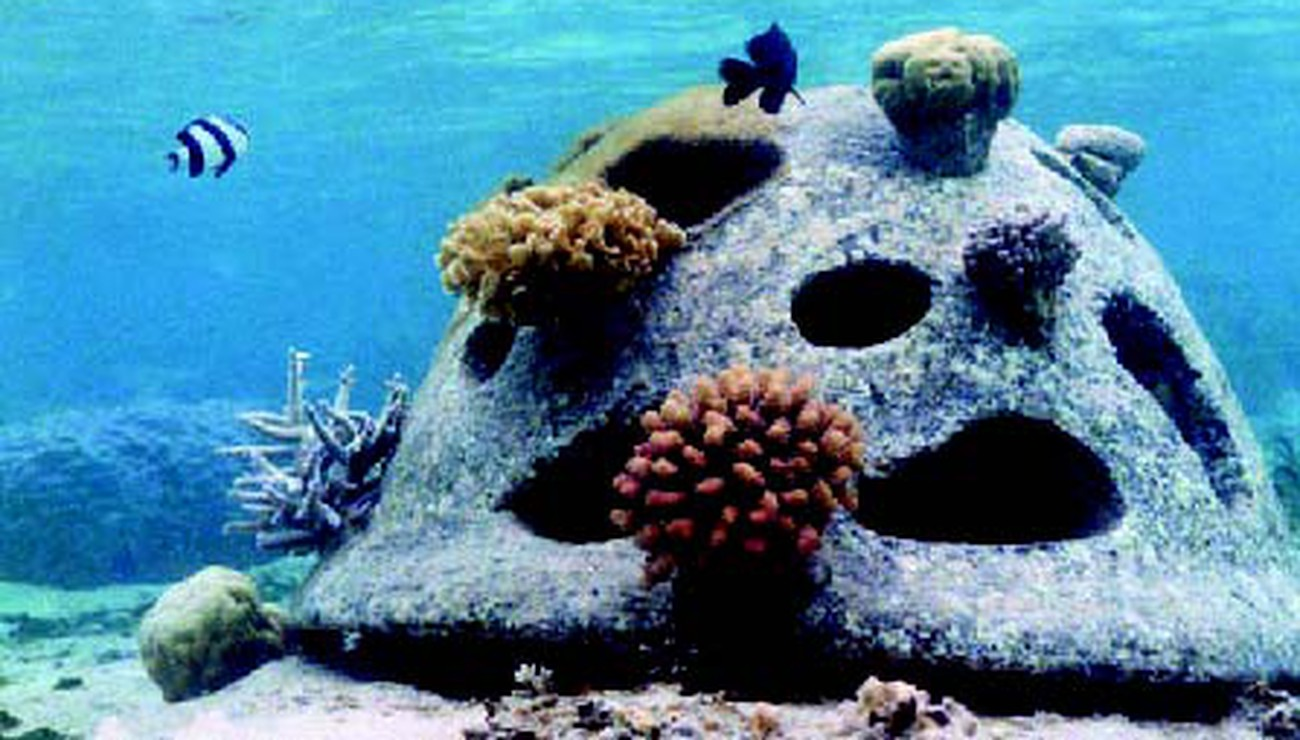
\includegraphics[width=0.6\linewidth]{images/recif} 

}

\caption{Figure 1 : Exemple de récif artificiel en béton}\label{fig:unnamed-chunk-2}
\end{figure}

\hypertarget{matuxe9riel-et-muxe9thodes}{%
\subsubsection{Matériel et méthodes }\label{matuxe9riel-et-muxe9thodes}}

\begin{enumerate}
\def\labelenumi{\arabic{enumi})}
\tightlist
\item
  L'atelier pédagogique
\end{enumerate}

Une première phase du programme pédagogique a été menée, à Paris, avec
les écoliers de primaire de Bondy. Deux ateliers ont été mis en place
pour l'étude : un atelier de bouturage et un atelier de prise de photos.
Dans un premier temps, les enfants ont fragmenté une colonie de
\emph{Slylophora sp.} à l'aide d'une pince coupante pour obtenir 12
boutures de corail branchu. Celles-ci ont ensuite été collées sur des
plots en céramique blanc, utilisés comme support
(\protect\hyperlink{Annexeux5cux25202}{Annexe 2}). Entre chaque coupe,
la colonie est gardée dans un bassin contenant l'eau de son aquarium,
afin de ne pas induire un stress supplémentaire qui pourrait
compromettre la survie des fragments. Un système de studio portatif est
conçu de sorte à réaliser une prise de photos exploitables pour le
traitement photogrammétrique. Un plateau tournant \emph{cablematic},
dont l'angle de rotation est commendable manuellement grâce à une
télécommande, est placé au centre d'une chambre ouverte en toile blanche
\emph{BeMatik}, réfléchissant la lumière. De part et d'autre, sont
installées les deux lampes associées au kit de studio photo
\emph{BeMatik} avec leur ampoules de 35W. Un appareil photo numérique
Sony RX 100 IV est posé sur un trépier devant l'ouverture de la chambre,
à une distance de \ldots{}. cm du plateau \emph{cablematic}. Les
boutures sont successivement photographiées sous différents angles. Le
pied du plot en céramique est imbriqué dans un trou d'un morceau de
grille en plastique pour être maintenu au centre du plateau tournant. On
définit un angle de rotation de \ldots{}° sur la télécommande. \ldots{}
photos du fragment sont alors prises à distance, avec l'appareil
commandé par un smartphone via une connection wifi. (Quelques images
sont aussi prises du dessus de la bouture?). Les coraux sont replacés
dans un bassin, une fois que la prise de photos est effectuée. Les
ateliers ont été menés en décembre 2021 et un renouvellement est prévu
pour le mois de mai 2022, afin d'effectuer le suivi de la croissance des
branches de \emph{Slylophora sp.}.

\begin{enumerate}
\def\labelenumi{\arabic{enumi})}
\setcounter{enumi}{1}
\tightlist
\item
  Reconstruction 3D
\end{enumerate}

La reconstruction en 3 dimensions des boutures de coraux s'effectue en
quelques grandes étapes avec Agisoft Metashape Professional version
1.5.1 (logiciel) (\protect\hyperlink{Annexeux5cux25201}{Annexe 1}).
Après le chargement de la série de photos, une première étape consiste à
estimer leur qualité. Dans le protocole de Lange et Perry, une qualité
est inférieure à 0,3 n'est pas suffisante pour que les photos soient
utilisées pour la modélisation (Lange and Perry 2020). Celles-ci sont
alors supprimées et les autres sont gardées afin de procéder à
``l'alignement''. Ce traitement consiste à faire correspondre les images
les unes avec les autres en les suturant avec leurs points semblables,
détectés par le logiciel ou déterminés à la main
(\protect\hyperlink{fig:Figureux5cux25202}{Figure 2}). Il s'agit souvent
de points remarquables comme une petite tâche isolée par exemple. Le
logiciel détecte ainsi quelles images se recouvrent partiellement. Le
mode ``Générique'' est appliqué lorsque, comme ici, les photos ne sont
pas géoréférencées.

\begin{figure}

{\centering 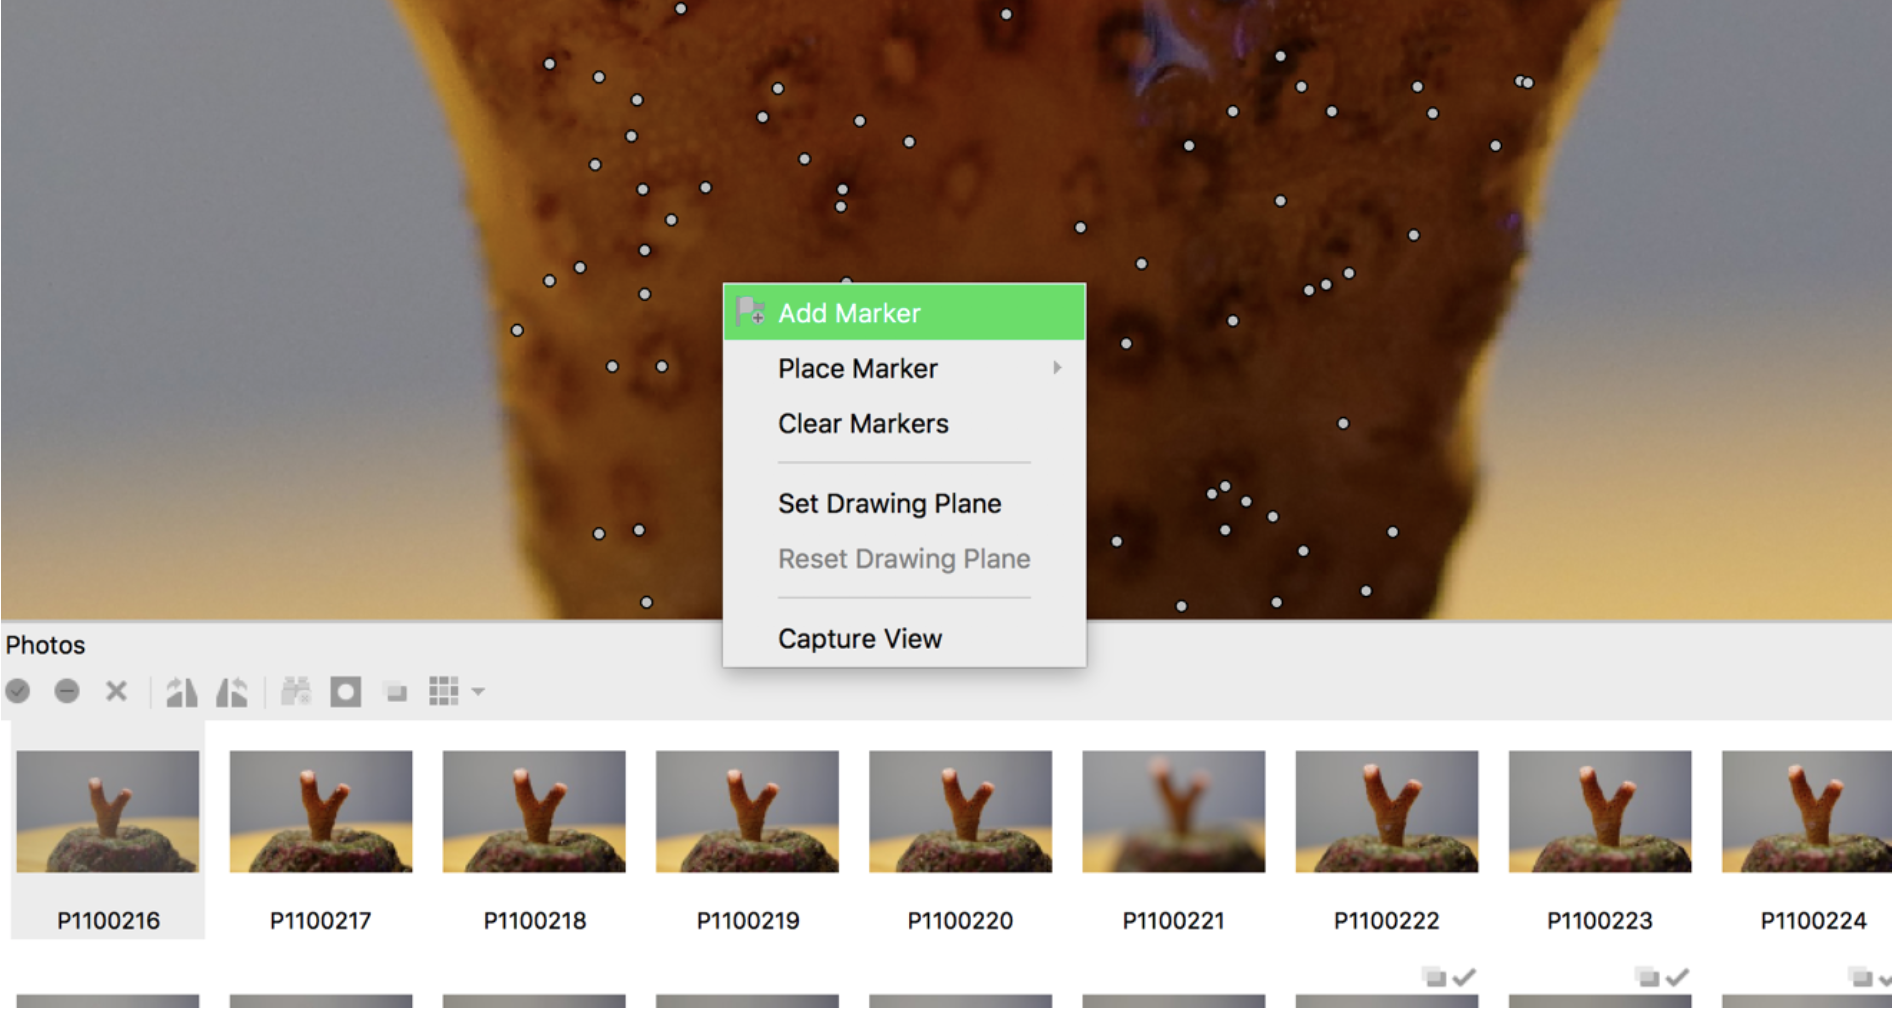
\includegraphics[width=0.6\linewidth]{images/metashape} 

}

\caption{Figure 2 : Ajoût manuel d'un point d'alignement sur Metashape Pro}\label{fig:unnamed-chunk-3}
\end{figure}

Cette étape du traitement est la seule sur laquelle une action peut être
effectuée manuellement afin d'optimiser le rendu de la reconstruction
3D. En choisissant une haute précision (relative au nombre de points),
le processus est plus lent mais on priorise la bonne estimation de la
position des photos, conservées avec leur nombre originel de pixels.
Après cette étape, les erreurs potentielles dans la reconstruction sont
réduites en supprimant les points au-dessus/en dessous de certains
niveaux d'incertitude et de précision. Plusieurs étapes successives de
suppression de points et d'optimisation de caméras permettent
d'atteindre l'objectif : réduire l'erreur (pix) à à 0,3--0,7 pour la
plupart des images et le nombre final de points dans le nuage à environ
10 000-15 000.

Metashape permet ensuite la création d'un nuage de points dense avec une
précision moyenne, réduisant le temps de traitement. La mise à l'échelle
est faite manuellement en ajoutant des marqueurs et en les associant à
deux points d'une règle, visible sur la photo. Il est possible de
générer un maillage de surface continu et texturé lorsque le modèle vise
à être utilisé dans des présentations. Pour des analyses de volumes ou
autre, c'est le nuage de points plus précis qui sera utilisé. Afin
d'estimer la précision de la modélisation 3D, on génère six modèles
supplémentaires pour chacune des boutures, à partir du même ensemble de
photos après en avoir retiré 10\% au hasard (d'après Ferrari et al.
(2017)). La précision (en mm) est calculée comme la distance moyenne
entre chacun des 6 nuages de points, construits et alignés sur celui
d'origine dans le logiciel CloudCompare version 2.10.2.

\begin{enumerate}
\def\labelenumi{\arabic{enumi})}
\setcounter{enumi}{2}
\tightlist
\item
  Automatisation avec R studio
\end{enumerate}

Un language python a déjà été créé par Metashape afin d'utiliser le
logiciel par ligne de commande et dans des programmes informatiques.
Ici, l'automatisation du processus de reconstruction 3D se basera sur la
création et le développement d'un package (ensemble de fonctions) pour
R, utilisable sur l'interface graphique Rstudio (RStudio Team 2015). Il
n'est pas envisagé que toutes les étapes de la modélisaion puissent être
automatisées. Cet algoritme permettra de commander les étapes de la
reconstruction qui ne nécessitent pas de réglages subjetives, comme
l'ajoût manuel de points d'alignement sur les photos. Ainsi, grâce aux
fonctions du packages, les utilisateurs pourront rapidement procéder à
l'ajoût de photos sur Metashape, l'estimation de la qualité des images
ou encore l'optimation des cameras
(\protect\hyperlink{Annexeux5cux25201}{Annexe 1}). Ce portage, après
avoir pris en main, nécessitera d'être complété par quelques fonctions
complémentaires pour l'automatisation d'étapes telles que la détection
d'automatique d'une règle pour la mise à l'échelle de l'objet.
L'efficacité de la technique sera testée, pour un échantillon de 3
boutures, grâce à une comparaison de la modélisation automatique avec la
méthode manuelle en suivant le protocol de Lange et Perry (Lange and
Perry 2020). L'objectif est d'atteindre le même degré de précision par
l'utilisation du package.

\hypertarget{annexes}{%
\subsubsection{Annexes}\label{annexes}}

Annexe 1

\begin{figure}

{\centering 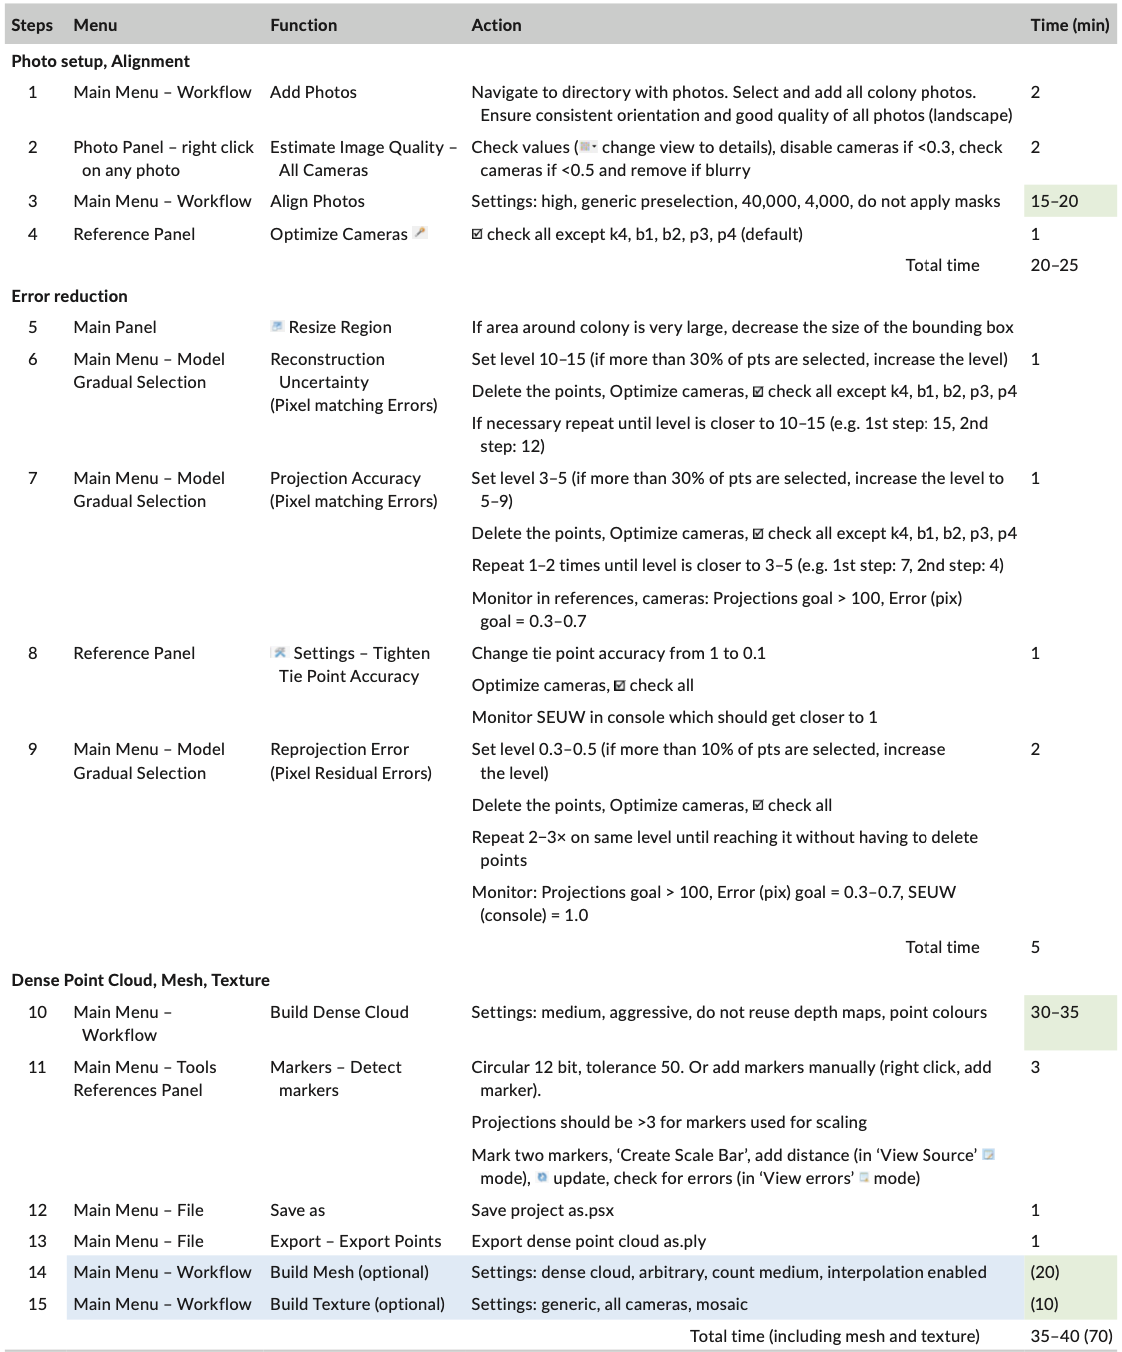
\includegraphics[width=0.6\linewidth]{images/protocol} 

}

\caption{Protole de reconstruction 3D sur Metashape Pro (Lange et Perry 2020)}\label{fig:unnamed-chunk-4}
\end{figure}

Annexe 2

\begin{figure}

{\centering 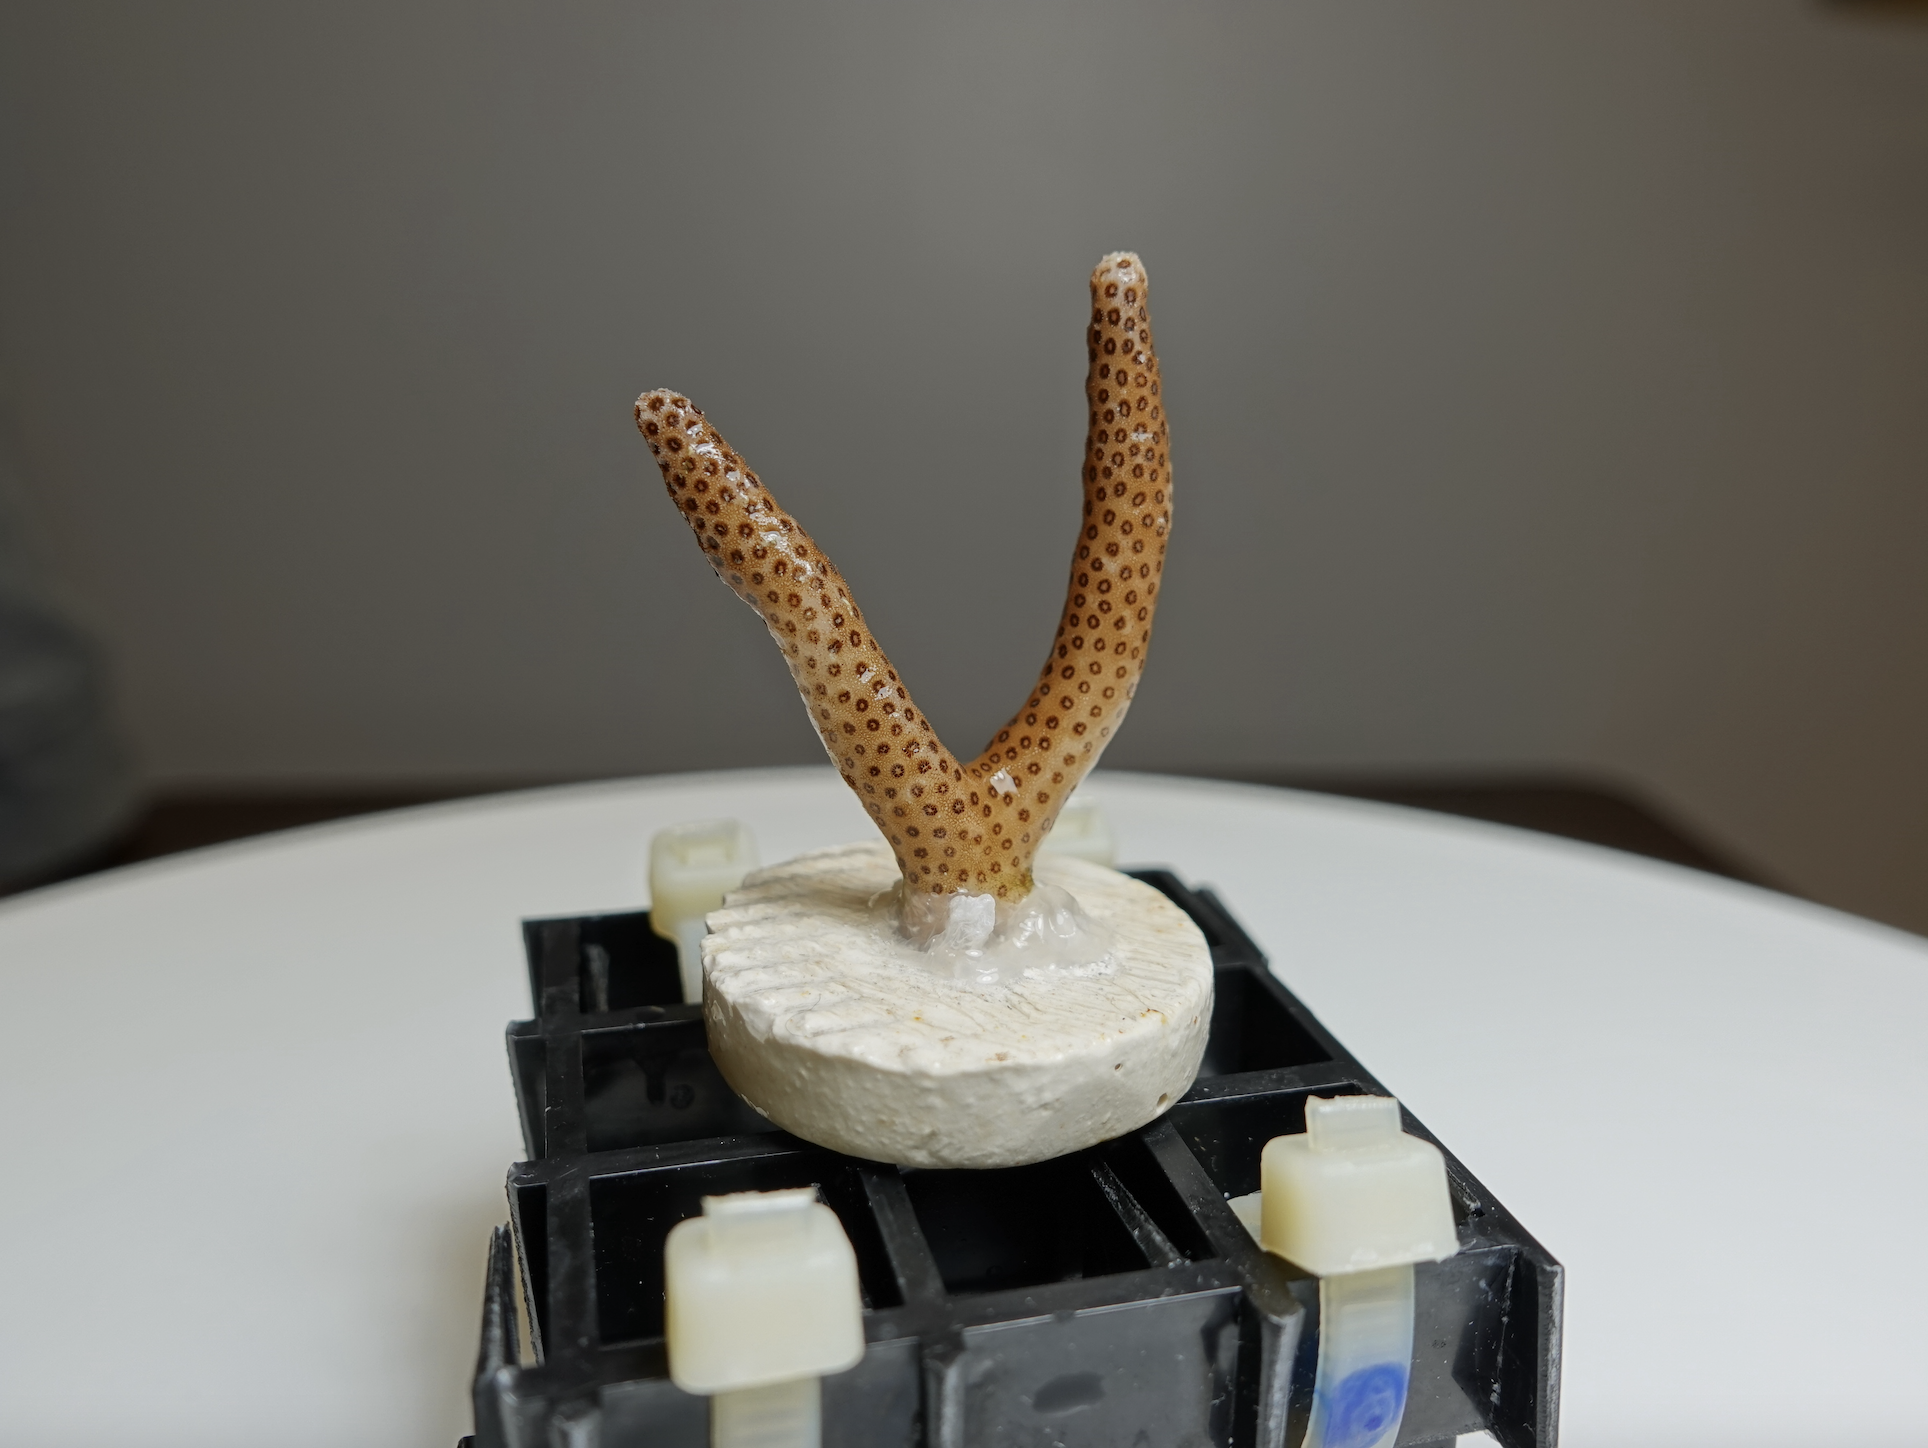
\includegraphics[width=0.6\linewidth]{images/bouture} 

}

\caption{Installatin d'une bouture de *Slylophora sp.* sur son support}\label{fig:unnamed-chunk-5}
\end{figure}

\hypertarget{ruxe9fuxe9rences}{%
\subsubsection*{Références}\label{ruxe9fuxe9rences}}
\addcontentsline{toc}{subsubsection}{Références}

\hypertarget{refs}{}
\leavevmode\hypertarget{ref-bensoussan_mer_2009}{}%
Bensoussan, Olivier. 2009. ``La Mer, Menace Ou Espoir de Développement
Pour Mayotte ?'' \emph{Les Cahiers d'Outre-Mer. Revue de Géographie de
Bordeaux} 62 (248): 489--512. \url{https://doi.org/10.4000/com.5779}.

\leavevmode\hypertarget{ref-cautain_future_2021}{}%
Cautain, Fanny. 2021. ``Future Maore Reef : La Mise En Place Des
Premiers Récifs Artificiels à Mayotte Parc Naturel Marin Mayotte.''
\emph{Parc Naturel Marin de Mayotte}, November.
\url{https://www.parc-marin-mayotte.fr/actualites/future-maore-reef-la-mise-en-place-des-premiers-recifs-artificiels-mayotte}.

\leavevmode\hypertarget{ref-comeau_resistance_2019}{}%
Comeau, S., C. E. Cornwall, T. M. DeCarlo, S. S. Doo, R. C. Carpenter,
and M. T. McCulloch. 2019. ``Resistance to Ocean Acidification in Coral
Reef Taxa Is Not Gained by Acclimatization.'' \emph{Nature Climate
Change} 9 (6): 477--83. \url{https://doi.org/10.1038/s41558-019-0486-9}.

\leavevmode\hypertarget{ref-coste_les_2021}{}%
Coste, Jean-François, Antoine Coursimault, Florent Brissaud, Jacques
Bongrand, Dominique Chauvin, and IESF. 2021. ``Les Prévisions Du GIEC.''
In \emph{Les Prévisions Du GIEC}, 21--24. EDP Sciences.
\url{https://doi.org/10.1051/978-2-7598-2250-8-005}.

\leavevmode\hypertarget{ref-darling_evaluating_2012}{}%
Darling, Emily S., Lorenzo Alvarez-Filip, Thomas A. Oliver, Timothy R.
McClanahan, and Isabelle M. Côté. 2012. ``Evaluating Life-History
Strategies of Reef Corals from Species Traits.'' \emph{Ecology Letters}
15 (12): 1378--86.
\url{https://doi.org/10.1111/j.1461-0248.2012.01861.x}.

\leavevmode\hypertarget{ref-diouf_volet_2016}{}%
Diouf, Papa Samba. 2016. ``Volet Adaptation Secteur Pêche,'' 68.

\leavevmode\hypertarget{ref-dokken_5_2014}{}%
Dokken, David. 2014. ``5 --- Coastal Systems and Low-Lying Areas,'' 49.

\leavevmode\hypertarget{ref-ferrari_3d_2017}{}%
Ferrari, Renata, Will F. Figueira, Morgan S. Pratchett, Tatiana Boube,
Arne Adam, Tania Kobelkowsky-Vidrio, Steve S. Doo, Trisha Brooke Atwood,
and Maria Byrne. 2017. ``3D Photogrammetry Quantifies Growth and
External Erosion of Individual Coral Colonies and Skeletons.''
\emph{Scientific Reports} 7 (1): 16737.
\url{https://doi.org/10.1038/s41598-017-16408-z}.

\leavevmode\hypertarget{ref-kapsenberg_coastal_2017}{}%
Kapsenberg, Lydia, Samir Alliouane, Frédéric Gazeau, Mousseau Laure, and
Jean-Pierre Gattuso. 2017. ``Coastal Ocean Acidification and Increasing
Total Alkalinity in the Northwestern Mediterranean Sea.'' \emph{Ocean
Science} 13 (May): 411--26.
\url{https://doi.org/10.5194/os-13-411-2017}.

\leavevmode\hypertarget{ref-lange_quick_2020}{}%
Lange, Ines D., and Chris T. Perry. 2020. ``A Quick, Easy and
Non-Invasive Method to Quantify Coral Growth Rates Using Photogrammetry
and 3D Model Comparisons.'' \emph{Methods in Ecology and Evolution} 11
(6): 714--26. \url{https://doi.org/10.1111/2041-210X.13388}.

\leavevmode\hypertarget{ref-mahafina_perception_2021}{}%
Mahafina, Jamal. 2021. ``Perception et Comportement Des Pêcheurs Pour
Une Gestion Durable de La Biodiversité et de La Pêcherie Récifale :
Application Au Niveau Des Réserves Marines Temporaires Du Sud Ouest de
Madagascar,'' 187.

\leavevmode\hypertarget{ref-olinger_growth_2019}{}%
Olinger, Lauren K., Alexander R. Scott, Steven E. McMurray, and Joseph
R. Pawlik. 2019. ``Growth Estimates of Caribbean Reef Sponges on a
Shipwreck Using 3D Photogrammetry.'' \emph{Scientific Reports} 9 (1):
18398. \url{https://doi.org/10.1038/s41598-019-54681-2}.

\leavevmode\hypertarget{ref-page_microfragmenting_2018}{}%
Page, Erinn et Vaughan, Christopher et Muller. 2018. ``Microfragmenting
for the Successful Restoration of Slow Growing Massive Corals.''
\emph{Ecological Engineering} 123 (September).
\url{https://doi.org/10.1016/j.ecoleng.2018.08.017}.

\leavevmode\hypertarget{ref-rstudio}{}%
RStudio Team. 2015. \emph{RStudio: Integrated Development Environment
for R}. Boston, MA: RStudio, Inc. \url{http://www.rstudio.com/}.

\leavevmode\hypertarget{ref-shaw_natural_2015}{}%
Shaw, Emily C., Stuart R. Phinn, Bronte Tilbrook, and Andy Steven. 2015.
``Natural in Situ Relationships Suggest Coral Reef Calcium Carbonate
Production Will Decline with Ocean Acidification.'' \emph{Limnology and
Oceanography} 60 (3): 777--88. \url{https://doi.org/10.1002/lno.10048}.

\leavevmode\hypertarget{ref-trebuil_resilience_2014}{}%
Trébuil, Par Guy. 2014. ``"Résilience \& Environnement : Pen- Ser Les
Changements Socio- écologiques" Raphaël Mathevet, François Bous- Quet -
Ed. Buchet-Chastel, Paris, Avril 2014, 170p.'' 3.

\leavevmode\hypertarget{ref-urbina-barreto_quantifying_2021}{}%
Urbina-Barreto, Isabel, Frédéric Chiroleu, Romain Pinel, Louis Fréchon,
Vincent Mahamadaly, Simon Elise, Michel Kulbicki, et al. 2021.
``Quantifying the Shelter Capacity of Coral Reefs Using Photogrammetric
3D Modeling: From Colonies to Reefscapes.'' \emph{Ecological Indicators}
121 (February): 107151.
\url{https://doi.org/10.1016/j.ecolind.2020.107151}.

\leavevmode\hypertarget{ref-veal_comparative_2010}{}%
Veal, C. J., G. Holmes, M. Nunez, O. Hoegh-Guldberg, and J. Osborn.
2010. ``A Comparative Study of Methods for Surface Area and
Three-Dimensional Shape Measurement of Coral Skeletons.''
\emph{Limnology and Oceanography: Methods} 8 (5): 241--53.
\url{https://doi.org/10.4319/lom.2010.8.241}.

\leavevmode\hypertarget{ref-wells_front_2006}{}%
Wells, Sue, and Corinna Ravilious. 2006. \emph{In the Front Line:
Shoreline Protection and Other Ecosystem Services from Mangroves and
Coral Reefs}. UNEP/Earthprint.

\leavevmode\hypertarget{ref-woolf_key_2019}{}%
Woolf, D.K., J.D. Shutler, L. Goddijn‐Murphy, A.J. Watson, B. Chapron,
P.D. Nightingale, C.J. Donlon, et al. 2019. ``Key Uncertainties in the
Recent Air‐Sea Flux of CO \(_{\textrm{2}}\).'' \emph{Global
Biogeochemical Cycles} 33 (12): 1548--63.
\url{https://doi.org/10.1029/2018GB006041}.

\end{document}
